\documentclass{article}
\usepackage{visionlab,xspace,tabularx}
\usepackage[margin=3cm]{geometry}
\usepackage{graphics}
\usepackage[usenames]{color}
%\usepackage{showkeys}
\usepackage{hyperref}

\newcommand{\x}{\mathbf{x}}

\title{An implementation of SIFT detector and descriptor}
\author{Andrea Vedaldi\\ University of California at Los Angeles}
\date{}

\definecolor{codecolor}{rgb}{0.1,0.8,0.0} 
\newcommand{\Matlab}{{\sc Matlab}\xspace}
\let\oldtt=\tt
\renewcommand{\tt}{\oldtt\color{codecolor}}

\begin{document}
\maketitle{}

% this will add all LaTeX labels as PDF destinations
% Used in combination with Hyperref, needs to be after \begin{document}
\let\oldlabel=\label
\renewcommand{\label}[1]{%
{\pdfdest name {#1} fitbh}% xyz
\oldlabel{#1}%
}

\tableofcontents{}

% ------------------------------------------------------------------------------
\section{Introduction}\label{sift.introduction}
% ------------------------------------------------------------------------------

These notes describe an implementation of the Scale-Invariant Transform Feature (SIFT) detector and descriptor \cite{lowe04distinctive}. The implementation is designed to produce results compatible to Lowe's version.\footnote{See {\tt http://www.cs.ubc.ca/\~ lowe/keypoints/}} Designed for the MATLAB environment, it is broken down into several M and MEX files that enable running only portion of the algorithm.

The SIFT {\em detector} extracts from an image a collection of {\em frames} or {\em keypoints}. These are oriented disks attached to blob-alike structures of the image. As the image translates, rotates and scales, the frames track these blobs and thus the deformation. By {\em canonization}, i.e. by mapping the frames to a reference (a canonical disk), the effect of such deformation on the feature appearance is removed.

The SIFT {\em descriptor} is a coarse description of the edge found in the frame. Due to canonization, descriptors are invariant to translations, rotations and scalings and are designed to be robust to residual small distortions.

The SIFT detector and descriptor are discussed in depth in~\cite{lowe04distinctive}. Here we only describe the interface to our implementation and, in the Appendix, some technical details.

% ------------------------------------------------------------------------------ 
\section{User reference: the {\tt sift} function}\label{sift.user}
% ------------------------------------------------------------------------------

The SIFT detector and the SIFT descriptor are invoked by means of the function {\tt sift}, which provides a unified interface to both.

\begin{example}[Invocation]
The following lines run the SIFT detector and descriptor on the image {\tt data/test.jpg}.
\begin{verbatim}
  I = imread('data/test.png') ;
  I = double(rgb2gray(I)/256) ;
  [frames,descriptors] = sift(I, 'Verbosity', 1) ;
\end{verbatim}
The pair option-value \verb$'Verbosity',1$ causes the function to print a detailed progress report.
\end{example}

The {\tt sift} function returns a $4\times K$ matrix {\tt frames} containing the SIFT frames and a $128 \times K$ matrix {\tt descriptors} containing their descriptors. Each frame is characterized by four numbers which are in order $(x_1,x_2)$ for the center of the frame, $\sigma$ for its scale and $\theta$ for its orientation. The coordinates $(x_1,x_2)$ are relative to the upper-left corner of the image, which is assigned coordinates $(0,0)$, and may be fractional numbers (sub-pixel precision). The scale $\sigma$ is the smoothing level at which the frame has been detected. This number can also be interpreted as size of the frame, which is usually visualized as a disk of radius $6\sigma$. Each descriptor is a vector describing coarsely the appearance of the image patch corresponding to the frame (further details are discussed in Appendix~\ref{sift.internals.descriptor}). Typically this vector has dimension 128, but this number can be changed by the user as described later.

Once frames and descriptors of two images $I_1$ and $I_2$ have been computed, {\tt siftmatch} can be used to estimate the pairs of matching features. This function uses Lowe's method to discard ambiguous matches~\cite{lowe04distinctive}. The result is a $2\times M$ matrix,  each column of which is a pair $(k_1,k_2)$ of indices of corresponding SIFT frames.
\begin{example}[Matching]
Let us assume that the images {\tt I1} and {\tt I2} have been loaded and processed as in the previous example. The code
\begin{verbatim}
  matches = siftmatch(descriptors1, descriptors2) ;
\end{verbatim}
stores in {\tt matches} the matching pairs, one per column.
\end{example}

The package provides some ancillary functions; you can
\begin{itemize}
\item use {\tt plotsiftframe} to plot SIFT frames;
\item use {\tt plotsiftdescriptor} to plot SIFT descriptors;
\item use {\tt plotmatches} to plot feature matches;
\item use {\tt siftread} to read files produced by Lowe's implementation.
\end{itemize}

\begin{example}[Visualization]
Let {\tt I1}, {\tt I2} and {\tt matches} be as in the previous example. To visualize the matches issue
\begin{verbatim}
  plotsiftmatches(I1,I2,frames1,frames2,matches)
\end{verbatim}
\end{example}

The {\tt sift} function has many parameters. The default values have been chosen to emulate Lowe's original implementation. Although our code does not result in frames and descriptors that are 100\% equivalent, in general they are quite similar.

% ------------------------------------------------------------------------------ 
\subsection{Scale space parameters}\label{sift.user.ss}
% ------------------------------------------------------------------------------ 

The SIFT detector and descriptor are constructed from the {\em Gaussian scale space} of the source image $I(x)$. The Gaussian scale space is the function
\[
   G(x;\sigma) \defeq (g_\sigma*I)(x)
\]
where $g_\sigma$ is an isotropic Gaussian kernel of variance $\sigma^2 I$, $x$ is the spatial coordinate and $\sigma$ is the scale coordinate. The algorithm make use of another scale space too, called {\em difference of Gaussian (DOG)}, which is, coarsely speaking, the scale derivative of the Gaussian scale space. 

Since the scale space $G(x;\sigma)$ represents the same information (the image $I(x)$) at different levels of scale, it is sampled in a particular way to reduce redundancy. The domain of the variable $\sigma$ is discretized in logarithmic steps arranged in $O$ octaves. Each octave is further subdivided in $S$ sub-levels. The distinction between octave and sub-level is important because at each successive octave the data is spatially downsampled by half. Octaves and sub-levels are identified by a discrete {\em octave index} $o$ and {\em sub-level index} $s$ respectively. The octave index $o$ and the sub-level index $s$  are mapped to the corresponding scale $\sigma$ by the formula
\be\label{eq:scale}
  \sigma(o,s) = \sigma_0 2^{o+s/S},
  \quad o \in o_{\min} + [0, ..., O-1],
  \quad s \in [0,...,S-1]
\ee
where $\sigma_0$ is the base scale level.

The {\tt sift} function accepts the following parameters describing the Gaussian scale space being used:
\begin{itemize}
\item {\tt NumOctaves}. This is the number of octaves $O$ in \eqref{eq:scale}.
\item {\tt FirstOctave}. Index of the first octave $o_{\min}$: the octave index $o$ varies in  $o_{\min},...,o_{\min}+O-1$. It is usually either $0$ or $-1$. Setting $o_{\min}$ to $-1$ has the effect of doubling the image before computing the Gaussian scale space.
\item {\tt NumLevels}. This is the number of sub-levels $S$ in \eqref{eq:scale}.
\item {\tt Sigma0}. Base smoothing: This is the parameter $\sigma_0$ in \eqref{eq:scale}.
\item {\tt SigmaN}. Nominal pre-smoothing: This is the nominal smoothing level of the input image. The algorithm assumes that the input image is actually $(g_{\sigma_n}*I)(x)$ as opposed to $I(x)$ and adjusts the computations according. Usually $\sigma_n$ is assumed to be half pixel (0.5).
\end{itemize}

% ------------------------------------------------------------------------------ 
\subsection{Detector parameters}\label{sift.user.detector}
% ------------------------------------------------------------------------------ 

The SIFT frames $(x,\sigma)$ are points of local extremum of the DOG scale space. The selection of such points is controlled by the following parameters:
\begin{itemize}
\item {\tt Threshold}. Local extrema threshold. Local extrema whose value $|G(x,;\sigma)|$ is below this number are rejected.
\item {\tt EdgeThreshold}. Local extrema localization threshold. If the local extremum is on a valley, the algorithm discards it as it is too unstable. Extrema are associated with a score proportional to their sharpness and rejected if the score is below this threshold.
\item {\tt RemoveBoundaryPoints}. Boundary points removal. If this parameter is set to 1 (true), frames which are too close to the boundary of the image are rejected.
\end{itemize}

% ------------------------------------------------------------------------------ 
\subsection{Descriptor parameters}\label{sift.user.descriptor}
% ------------------------------------------------------------------------------ 

The SIFT descriptor is a weighted and interpolated histogram of the gradient orientations and locations in a patch surrounding the keypoint. The descriptor has the following parameters:
\begin{itemize}
\item {\tt Magnif}. Magnification factor $m$. Each spatial bin of the histogram has support of size $m \sigma$, where $\sigma$ is the scale of the frame.
\item {\tt NumSpatialBins}. Number of spatial bins. Together with the next parameter, this number defines the extension and dimension of the descriptor. The dimension of the descriptor (the total number of bins) is equal to
$\mathtt{NumSpatialBins}^2 \times \mathtt{NumOrientBins}$ and its extension (the patch where the gradient statistic is collected) has radius $\mathtt{NumSpatialBins} \times m\sigma/2$. 
\item {\tt NumOrientBins}. Number of orientation bins.
\end{itemize}

% ------------------------------------------------------------------------------ 
\subsection{Direct access to SIFT components}\label{sift.user.direct}
% ------------------------------------------------------------------------------ 

The SIFT code is decomposed in several M and MEX files, each implementing a portion of the algorithm. These programs can be run on their own or replaced. Appendix~\ref{sift.internals} contains information useful to do this.


\begin{example}[Computing the SIFT descriptor directly]
Sometimes it is useful to run the descriptor code alone.
This can be done by calling the function {\tt siftdescriptor} (which is actually a MEX file.) See the function help for further details.
\end{example}

% ------------------------------------------------------------------------------ 
\bibliographystyle{plain}
\bibliography{bibliography}
% ------------------------------------------------------------------------------

\appendix
% ------------------------------------------------------------------------------ 
\section{Internals}\label{sift.internals}
% ----------------------------------------------------------------------------- 

% ------------------------------------------------------------------------------ 
\subsection{Scale spaces}\label{sift.internals.ss}
% ------------------------------------------------------------------------------
\begin{figure}
\begin{center}
\begin{tabular}{lp{0.4\textwidth}p{0.3\textwidth}}
\hline
\bf Symbol & \bf Description & \bf In the code
\\\hline
$o\in[o_{\min},o_{\min}+O-1]$ & Octave index and range & \tt o, O, omin
\\
$s\in[s_{\min},s_{\max}]$   & Scale index and range &  \tt s, smin, smax
\\
$\sigma(o,s) = \sigma_02^{o + s/S}$ & Scale coordinate formula &
\\
$\sigma_0$ & Base scale offset & \tt sigma0
\\
$M_0,$ $N_0$ & Base spatial resolution (octave $o=0$) &
\\
$N_o = \lfloor \frac{N_0}{2^o}\rfloor,$
$M_o = \lfloor \frac{M_0}{2^o}\rfloor$
& Octave lattice size formulas &
\\
$x_o \in [0,...,N_o]\times[0,...,M_o]$ & Spatial indexes and rages &
\\
$x = 2^o x_o$ & Spatial coordinate formula
\\
$F(\cdot,\sigma(o,\cdot))$ & Octave data & \tt octave
\\
$G(x,\sigma)$ & Gaussian scale space & \tt gss
\\
$D(x,\sigma)$ & DOG scale space & \tt dogss
\\\hline
\end{tabular}
\end{center}
\caption{{\sl Scale space parameters.} The SIFT descriptors uses two scale spaces: a Gaussian scale space and a Difference of Gaussian scale space. Both are described by these parameters.}\label{tab:ssparam}
\end{figure}

Here a {\em scale space} is a function $F(x,\sigma) \in \real$ of a spatial coordinate $x\in\real^2$ and a scale coordinate $\sigma\in\real_+$. Since a scale space $F(\cdot,\sigma)$ typically represents the same information at various scales $\sigma\in\real$, its domain is sampled in a particular way in order to reduce the redundancy.

The scale coordinate $\sigma$ is discretized in logarithmic steps according to
\[
   \sigma(s,o) = \sigma_0 2^{o + s/S}, 
   \qquad o\in\integer,
   \quad s=0,...,S-1
\]
where $o$ is the {\em octave index}, $s$ is the {\em scale index}, $S\in \naturalnumber$ is the {\em scale resolution} and $\sigma_0\in\real_+$ is the {\em base scale offset}. Note that it is possible to have octaves of negative index.

The spatial coordinate $x$ is sampled on a lattice with a resolution which is a function of the octave. We denote $x_o$ the spatial index for octave $o$; this index is mapped to the coordinate $x$ by
\[
  x = 2^o x_o, 
  \qquad o\in\integer,
  \quad x_o \in [0,...,N_o-1]\times[0,...,M_o-1].
\] 
where $(N_o,M_o)$ is the spatial resolution of octave $o$. If $(M_0,N_0)$ is the the resolution of the base octave $o=0$, the resolution of the other octaves is obtained as
\[
 N_o = \lfloor \frac{N_0}{2^o}\rfloor,
 \qquad
 M_o = \lfloor \frac{M_0}{2^o}\rfloor.
\]

It will be useful to store some scale levels twice, across different octaves. We do this by allowing the parameter $s$ to be negative or greater than $S$. Formally, we denote the range of $s$ as $[s_{\min},s_{\max}]$. We also denote the range of the octave index $o$ as $[o_{\min},o_{\min}+O-1]$, where $O\in\naturalnumber$ is the total number of octaves. See Figure~\ref{tab:ssparam} for a summary of these symbols.

The SIFT detector makes use of the two scale spaces described next.

\medskip
\noindent{\bf Gaussian Scale Space.} The {\em Gaussian scale space} of an image $I(x)$ is the function
\[
   G(x,\sigma) \defeq (g_\sigma * I)(x)
\]
where the scale $\sigma = \sigma_0 2^{o+s/S}$ is sampled as explained in the previous section. This scale space is computed by the function {\tt gaussianss}. In practice, it is assumed that the image passed to the function 
{\tt gaussianss} is already pre-smoothed at a nominal level $\sigma_n$, so that 
$G(x,\sigma) = (g_{\sqrt{\sigma^2 - \sigma_n^2}} * I)(x)$. As suggested in
\cite{lowe04distinctive}, the pyramid is computed incrementally from the bottom by successive convolutions with small kernels.

\medskip
\noindent{\bf Difference of Gaussians scale space.} The {\em difference of Gaussians (DOG) scale space} is the scale ``derivative'' of the Gaussian scale space $G(x,\sigma)$ along the scale coordinate $\sigma$. It is given by
\[
  D(x,\sigma(s,o)) \defeq G(x,\sigma(s+1,o)) - G(x,\sigma(s,o)).
\]
It is obtained from the Gaussian scale space by the {\tt diffss} function.

\begin{remark}[Lowe's parameters] Lowe's implementation uses the following parameters:
\[
\sigma_n = 0.5,
\quad
\sigma_0 = 1.6\cdot 2^{1/S},
\quad
o_{\min} = -1,
\quad
S =3
\]
In order to compute the octave $o=-1$, the image is doubled by bilinear interpolation (for the enlarged image $\sigma_n=1$). In order to detect extrema at all scales, the Difference of Gaussian scale space has $s\in[s_{\min},s_{\max}]=[-1,S]$. Since the Difference of Gaussian scale space is obtained by differentiating the Gaussian scale space, the latter has
$s\in[s_{\min},s_{\max}] = [-1,S+1]$. The parameter $O$ is set to cover all octaves (i.e. as big as possible.)
\end{remark}

% ------------------------------------------------------------------------------ 
\subsection{The detector}\label{sift.internals.detector}
% ------------------------------------------------------------------------------

The SIFT frames (or ``keypoints'') are a selection of (sub-pixel interpolated) points $(x,\sigma)$ of local extremum of the DOG scale-space $D(x,\sigma)$, together with an orientation $\theta$ derived from the spatial derivative of the Gaussian scale-space $G(x,\sigma)$. For what concerns the detector (and being in general different for the descriptor), the ``support'' of a keypoint $(x,\sigma)$ is a Gaussian window $H(x)$ of deviation $\sigma_w=1.5\sigma$. In practice, the window is truncated at $|x|\leq 4 \sigma_w$.

The Gaussian and DOG scale spaces are derived as in Section~\ref{sift.internals.ss}. In this Section, the parameters $S,$ $O,$ $s_{\min},$ $s_{\max},$ $o_{\min},$ $\sigma_0$ refer to the DOG scale space. The Gaussian scale space has exactly the same parameters of the DOG scale space except for $s_{\max}^{\text{DOG}}$ which is equal to $s_{\max} - 1$.

The extraction of the keypoints is carried one octave per time and articulated in the following steps:

\begin{itemize}
\item {\bf Detection.} Keypoints are detected as points of local extremum of $D(x,\sigma)$ (Section~\ref{sift.internals.ss}). In the implementation the function {\tt siftlocalmax} extracts such extrema by looking at $9\times 9 \times 9$ neighborhoods of samples.

As the octave is represented by a 3D array, the function {\tt siftlocalmax} returns indexes $k$ (in \Matlab convetion) that are to be mapped to scale space indexes $(x_1,x_2,s)$ by
\[
  k-1 = x_2 + x_1 M_o + (s-s_{\min}) M_o N_o.
\]
Alternatively, one can use {\tt ind2sub} to map the index $k$ to a subscript $(i,j,l)$ and then use
\[
  x_1=j-1, \qquad
  x_2=i-1, \qquad
  s=l-1+s_{\min}.
\]
Because of the way such maxima are detected, one has always
$1\leq x_2 \leq M_o-2,$ $1\leq x_1 \leq N_o-2$ and $s_{\min}+1\leq s \leq s_{\max}-1$. 

Since we are interested both in local maxima and minima, the process is repeated for $-G(x,\sigma)$. (If only positive maxima and negative minima are of interest, another option is to take the local maxima of $|G(x,\sigma)|$ directly, which is quicker.)

%%
\item {\bf Sub-pixel refinement.} After being extracted by {\tt siftlocalmax}, the index $(x_1,x_2,s)$ is fitted to the local extremum by quadratic interpolation. At the same time, a threshold on the ``intensity'' $D(x,\sigma)$ and a test on the ``peakedness'' of the extremum is applied in order to reject weak points or points on edges. These operations are performed by the {\tt siftrefinemx} function. 

The edge rejection step is explained in detail in the paper \cite{lowe04distinctive}. The sub-pixel refinement is an instance of Newton's algorithm.


%%
\item {\bf Orientation.} The orientation $\theta$ of a keypoint $(x,\sigma)$ is
obtained as the predominant orientation of the gradient in a window around the keypoint. The predominant orientation is obtained as the (quadratically interpolated) maximum of the histogram of the gradient orientations $\angle \nabla G(x_1,x_2,\sigma)$ within a window around the keypoint. The histogram is weighted both by the magnitude of the gradient $|\nabla G(x_1,x_2,\sigma)|$ and a Gaussian window centered on the keypoint and of deviation $1.5\sigma$ (the Gaussian window defines the region of interest as well). After collecting the data in the bins and before computing the maximum, the histogram is smoothed by a moving average filter.

In addition to the global maximum, each local maximum with a value above 0.8\% of the maxium is retained as well. Thus for each location and scale multiple SIFT frames might be generated.

These computations are carried by the function {\tt siftormx}.

\end{itemize}

% ------------------------------------------------------------------------------ 
\subsection{The descriptor}\label{sift.internals.descriptor}
% ------------------------------------------------------------------------------

\begin{figure}
\begin{center}
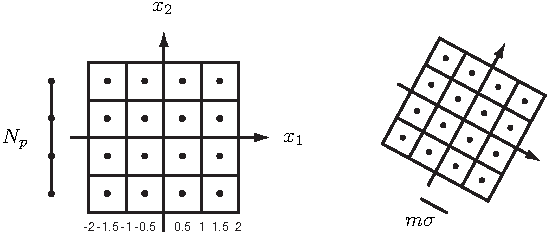
\includegraphics{figures/sift-descriptor}
\end{center}
\caption{{\sl SIFT descriptor layout.} The actual size of a spatial bin is $m\sigma$ where $\sigma$ is the scale of the keypoint and $m=3.0$ is a nominal factor.}\label{fig:descriptor}
\end{figure}

The SIFT descriptor of a keypoint $(x,\sigma)$ is a local statistic of the orientations of the gradient of the Gaussian scale space $G(\cdot,\sigma)$.

\medskip
\noindent{\bf Histogram layout.} The SIFT descriptor (Figure~\ref{fig:descriptor}) is an histogram of the gradient orientations augmented and {2-D} locations in the support of the SIFT frame. Formally, the domain of the histogram are the tuples $(x,\theta)\in \real^2 \times \real/\integer$. The bins form a three dimensional lattice with $N_p=4$ bins for each spatial direction and $N_o=8$ bins for the orientation for a total of $N_p^2 N_o=128$ components (these numbers can be changed by setting the appropriate parameters). Each spatial bin is square with unitary edge. The window $H(x)$ is Gaussian with deviation equal to half the extension of the spatial bin range, that is $N_p/2$.

\medskip
\noindent{\bf Keypoint normalization.} In order to achieve invariance, the histogram layout is projected on the image domain according to the frame of reference of the keypoint. The spatial dimensions are multiplied by $m\sigma$ where $\sigma$ is the scale of the keypoint and $m$ is a nominal factor (equal to 3.0 by default). The layout is also rotated so that the axis $x_1$ is aligned to the direction $\theta$ of the keypoint.

\medskip
\noindent{\bf Weighting.} The histogram is weighted by the gradient modulus and a Gaussian windowed and tri-linearly interpolated. More in detail, each sample $(x_1,x_2,\angle\nabla G(x,\sigma))$ is
\begin{itemize}
\item weighted by $|\nabla G(x,\sigma)|$;
\item weighted by the gaussian window $H(x)$;
\item projected on the centers of the eight surrounding bins;
\item summed to each of this bins proportionally to its distance from the respective center.
\end{itemize}

\begin{remark}(Lowe's impelmentation)
In order to achieve full compatibility with Lowe's original implementation, one needs to pay attention to many little details as the memory layout of the descriptor and the convention for the gradient orientations. These are detailed in the source code.
\end{remark}

\end{document}
